As mentioned in section~\ref{subsec:userinterface} Google Glass is equipped with a camera that could be used to take photos from the user's perspective. One potential use of the camera would be to scan Quick Response (QR) codes. The QR Code was announced in 1994. Having been under development for several years at Denso Wave~\cite{qrCodeHistory} the goal was to create a new form of barcode that could carry more information than a linear barcode and be easily read.

A conventional barcode is capable of storing approximately 20 digits while a QR code can store several thousand digits~\cite{qrCodeType}. Information is encoded using standardised encoding modes and displayed as a 2D barcode. A QR code has several standardised fields, as seen in Figure~\ref{qrcodestandard}. Using position fields a QR code can be read from any direction, compared to a conventional barcode which can only be read horizontally~\cite{qrCodeAbout}.

	\begin{figure}[H]%ht!]
		\centering
		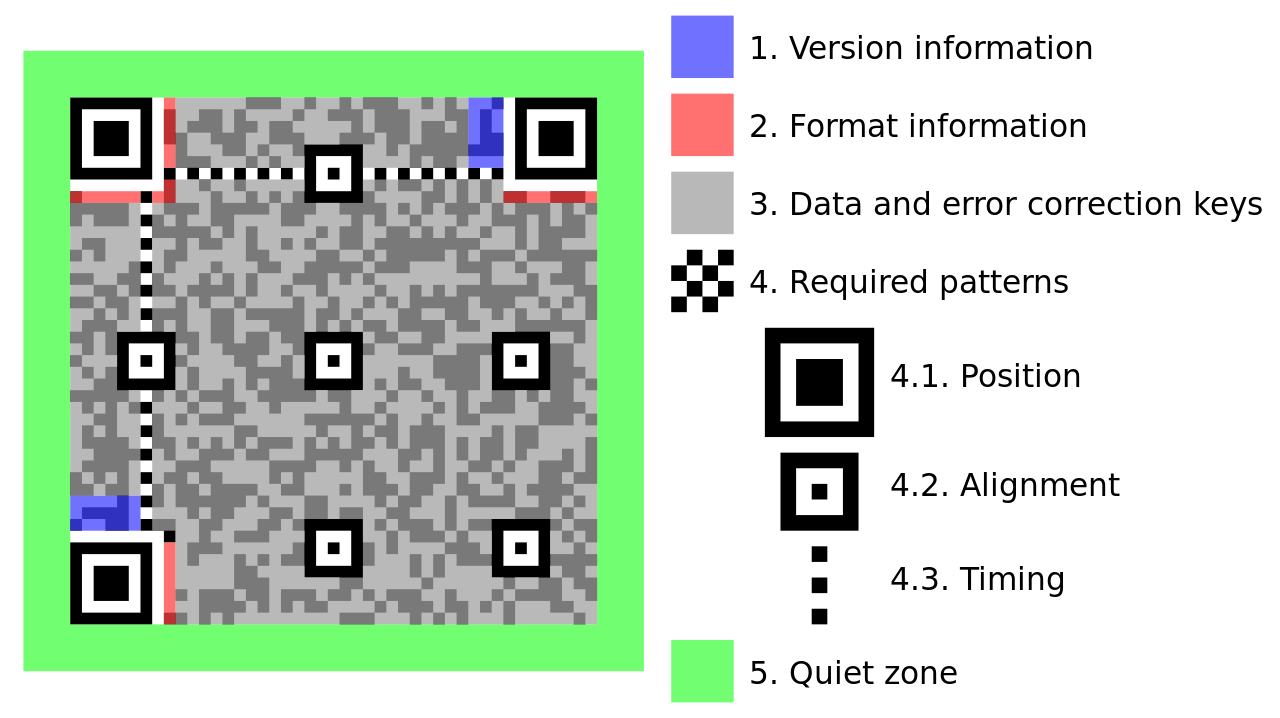
\includegraphics[width=110mm]{images/qrcodestandard}
		\caption{The standardised fields in a QR Code~\cite{qrCodeWiki}.}
		\label{qrcodestandard}
	\end{figure}
	 
A QR code can be used to encode information, originally written with alphabetic characters, japanese symbols (Kanji) or numeric characters~\cite{qrCodeVersion}. With the help of a QR code information which would otherwise have taken up a large space can now be easily fitted in smaller areas.